% \edo{I think having a high-level quick description of the different phases (parent sampling, inspiration sampling, program mutation, filtering , ... etc. would help better contextualize each before diving in the details)} - this is a preliminary sketch
\textbf{Algorithm Overview.} \ouralgo's control-flow entails three main phases: 
\begin{enumerate}
\item \textit{Parent and inspiration sampling} from an archive of island program subpopulations. Importantly, we emphasize the trade-off between exploration and exploitation in parent program selection.
\item \textit{Program mutation} via LLM-guided code edit proposals. We utilize novelty rejection-sampling based on code embedding similarity and an LLM-as-a-novelty-judge assessment.
\item \textit{Program execution and world feedback} guiding the LLM ensemble selection probabilities and online meta-scratchpad drafting for documentation and knowledge diffusion.
\end{enumerate}

\subsection{Parent and inspiration sampling}
\textbf{Archive Maintenance, Island Populations \& Mutation Context Construction}. \ouralgo maintains a fixed-size archive of previously evaluated programs with fitness scores and meta information, implementing an elite size constraint. The mutation context incorporates a primary parent program alongside inspiration programs drawn from top-performing solutions and random archive samples, providing the LLM with diverse exemplars for creative recombination. We follow \citet{romera2024mathematical,novikov2025alphaevolve} and employ an island model approach with independent subpopulations seeded from the same initial program. The islands evolve in parallel to enhance diversity and prevent premature convergence. Island members can occasionally migrate between islands to diffuse knowledge across ``discovery substreams''. To protect the uniqueness of each island, we prevent the island-specific best-performing program from migrating~\citep{tanese1989distributed, romera2024mathematical}. Sampling occurs hierarchically: with the island ID first sampled uniformly from the archive, later used as the origin for both parent and inspirations. Afterwards, we sample random archive programs and the top-K performing programs to use them as context programs.

\textbf{Balancing Exploration \& Exploitation: Parent Program Selection}. Given an island subpopulation, \ouralgo implements multiple different parent sampling strategies that balance exploration and exploitation: 
%
First, we employ power law sampling where programs are ranked by fitness with ranks $r_i$ ($r_i = 1$ for the best program). The selection probability follows $p_i = \frac{r_i^{-\alpha}}{\sum_{j=1}^{n} r_j^{-\alpha}}$, where $\alpha$ controls exploitation intensity. Setting $\alpha = 0$ yields uniform sampling, while $\alpha \to \infty$ implements hill-climbing.
%
Inspired by \citet{zhang2025darwin}, we contrast this with weighted sampling, incorporating performance and novelty. Given programs with offspring count $N(P_i)$, we first compute the median fitness $\alpha_0 = \text{median}(\{F(P_1), F(P_2), ..., F(P_n)\})$. The performance component uses sigmoid scaling: $s_i = \sigma(\lambda \cdot (F(P_i) - \alpha_0))$ where $\sigma(x) = \frac{1}{1 + e^{-x}}$ and $\lambda$ controls selection pressure. The novelty component $h_i = \frac{1}{1 + N(P_i)}$ favors programs with fewer offspring. The final probability combines these: $p_i = \frac{w_i}{\sum_{j=1}^{n} w_j}$ where $w_i = s_i \cdot h_i$ balances performance and novelty. The strategies are illustrated in \Cref{fig:parent_sampling}.

\begin{figure}[h!]
    \centering
    
\includegraphics[width=0.925\textwidth]{figures/f2_a_sampling.pdf}
    \caption{\textbf{\ouralgo Parent Sampling.} The strategies range from pure exploration (uniform sampling) to pure exploitation (hill-climbing) to a combination of performance and novelty.}
    \label{fig:parent_sampling}
    % \vspace{-15pt}
\end{figure}


\subsection{Program mutation and novelty assessment}

\textbf{LLM-Guided Program Mutations}.  To generate new programs, \ouralgo starts by sampling a specific LLM and a set of sampling parameters (e.g., temperature or reasoning budget) from a pre-specified pool. Our framework provides support for models from leading API providers, including GPT, Gemini, Claude, and DeepSeek~\citep{gpt4, moe_gemini25, claude3, guo2025deepseek}. After sampling a model, \ouralgo employs three distinct mutation approaches to foster diversity and creativity in the LLM-generated program variants: 
%
\begin{enumerate}
\item \textbf{Diff-Based Edits.} We implement diff edits using LLMs following the approach outlined in \citet{novikov2025alphaevolve}, utilizing SEARCH/REPLACE blocks for targeted modifications.
\item \textbf{Full Rewrites.} We enable full program rewrites to allow greater flexibility, programmatically ensuring that non-mutable blocks remain unchanged during the LLM rewrite process. 
\item \textbf{Crossover Mutation.} We leverage crossover mutations \citep{lehman2022evolutionlargemodels,lange2025ai} where an additional archive program is sampled and an LLM is prompted to combine programs.
\end{enumerate}
%

Following \citet{novikov2025alphaevolve}, we use text markers (\texttt{EVOLVE-BLOCK-START} \& \texttt{EVOLVE-BLOCK-END}) to ensure that immutable code is left unchanged during the LLM rewrite process. After obtaining a code change proposal, we enforce that the immutable code is not touched and resample a new proposal if a patch is invalid, providing parsing feedback using Reflexion \citep{shinn2024reflexion}. 
% We provide a side-by-side comparison of the prompting structure for each mutation approach in Figure~\edo{I think a figure specific to this part would help, if space permits}.\rob{I disagree.}

% EDO: maybe introduce this as a 2-part filtering approach?
\textbf{Program Diversity via Novelty Rejection Sampling}. To enhance the creativity of executed code proposals, we leverage a foundation model ensemble combined with temperature sampling. Additionally, we introduce \textit{code novelty rejection sampling} using an embedding model to embed mutable parts of the program code. Afterwards, we compute cosine similarity scores across the island subpopulation programs. If the maximal score exceeds a threshold (e.g., $\eta=0.95$), we query an LLM to further assess whether the program is meaningfully different. The approach is illustrated in \Cref{fig:novelty_rejection_sampling}.

\begin{figure}[h!]
    \centering
    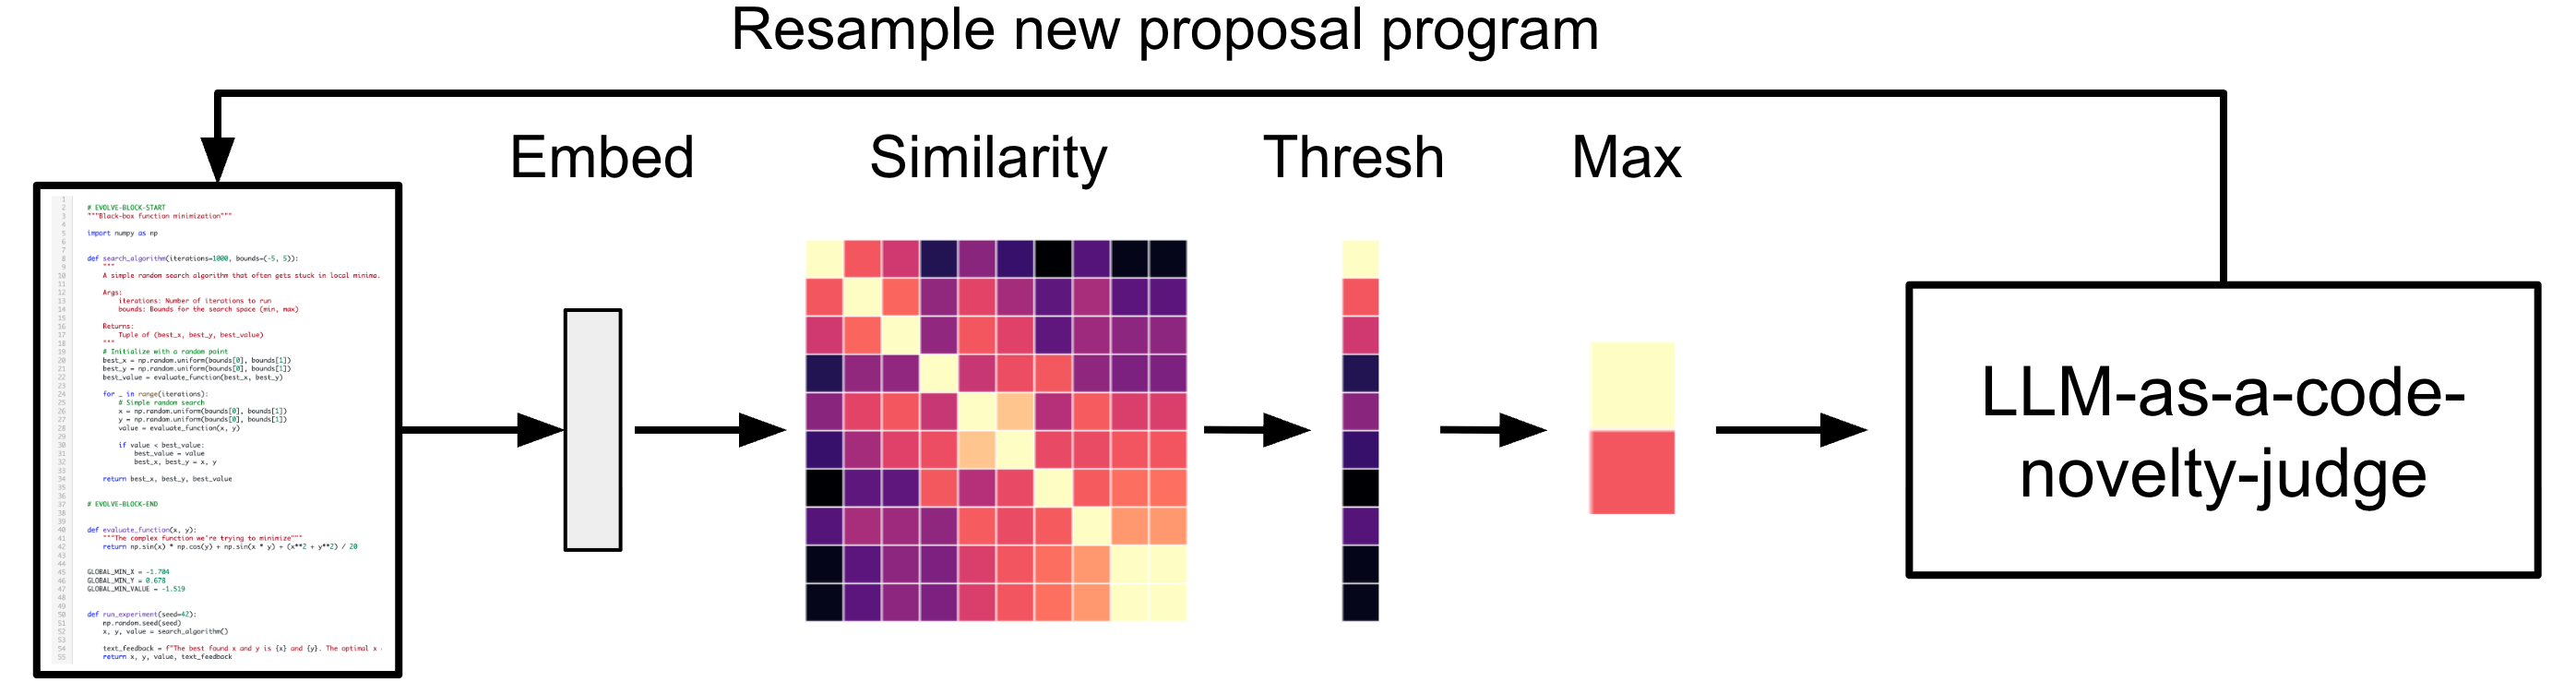
\includegraphics[width=0.925\textwidth]{figures/f2_b_rejection.png}
    \caption{\textbf{\ouralgo Program Novelty Rejection Sampling.} \ouralgo embeds mutable code snippets, computes similarities across the archive; if the maximal score exceeds a threshold, another LLM is queried to assess whether the program is meaningfully novel.}
    \label{fig:novelty_rejection_sampling}
\end{figure}

\subsection{Execution and world feedback}

\textbf{Multi-Objective Optimization \& Textual Feedback}. After a program obtained with the above steps is executed, \ouralgo performs multi-objective assessment yielding both its scalar fitness value $r_i$ together with a set of exposed ``public metrics'' and textual feedback. \ouralgo then stores this full multi-objective assessment in the population archive to provide an informative context for future generations of language model mutations using a simple prompting format:

\begin{tcolorbox}[breakable,colback=orange!5!white, colframe=orange!80!black, title=Example of Diff Edit Prompt with Textual Feedback]
\tiny
\begin{Verbatim}[breaklines=true,breakanywhere=true]
# Current program
Here is the current program we are trying to improve (you will need to propose a modification to it below):
```{language}
{code_content}
```
Here are the performance metrics of the program:
{performance_metrics}{text_feedback_section}

# Instructions
...
# Task
...
IMPORTANT: Do not rewrite the entire program - focus on targeted improvements.
\end{Verbatim}
\end{tcolorbox}

\textbf{Adaptive LLM sampling evolution}. The performance of different LLMs to propose mutations can vary across problem domains and based on the current state of the sampled archive parents and inspiration programs. \ouralgo dynamically adapts to this non-stationarity by evolving the LLM sampling probability throughout at the end of each generation. Our approach is based on the UCB1 algorithm~\citep{ucb_sem}, associating each LLM with a visitation counter and an estimate of the expected score updated with the performance of its sampled mutations. We introduce changes tailored to the domain of LLM-driven discovery. In particular, rather than the absolute fitness of each mutation $r_i$, we update the LLM distribution using: $r_i^u = \exp\!\left(\max(r_i - r_i^b, 0)\right) - 1$, where $r_i^b$ is the baseline reward for program $i$ computed as the maximum between its parent program and the initial program in the database, ensuring each LLM is evaluated based on its relative improvement to account for the non-stationarity of the program archive. At the same time, the $\exp(\cdot)$ and $\max(\cdot, 0)$ operations help precisely promote LLMs able to come up with bold, high-risk, high-reward mutations,  over ``safer'' minor improvements. We use the tracked statistics over the observed rewards to normalize $r_i^u$ and ensure invariance to the fitness scale of each domain.

\textbf{Meta-Scratchpad \& Online Refinement}. \ouralgo implements a meta-scratchpad system that periodically analyzes successful solutions to accelerate learning. Every $T$ generations, we summarize the recent program evaluations and identify common optimization strategies and design principles. The meta-agent synthesizes insights into actionable recommendations appended to the mutation prompt, providing high-level guidance from accumulated evolutionary experience. The approach is illustrated in \Cref{fig:meta_scratchpad}.

\begin{figure}[h!]
    \centering
    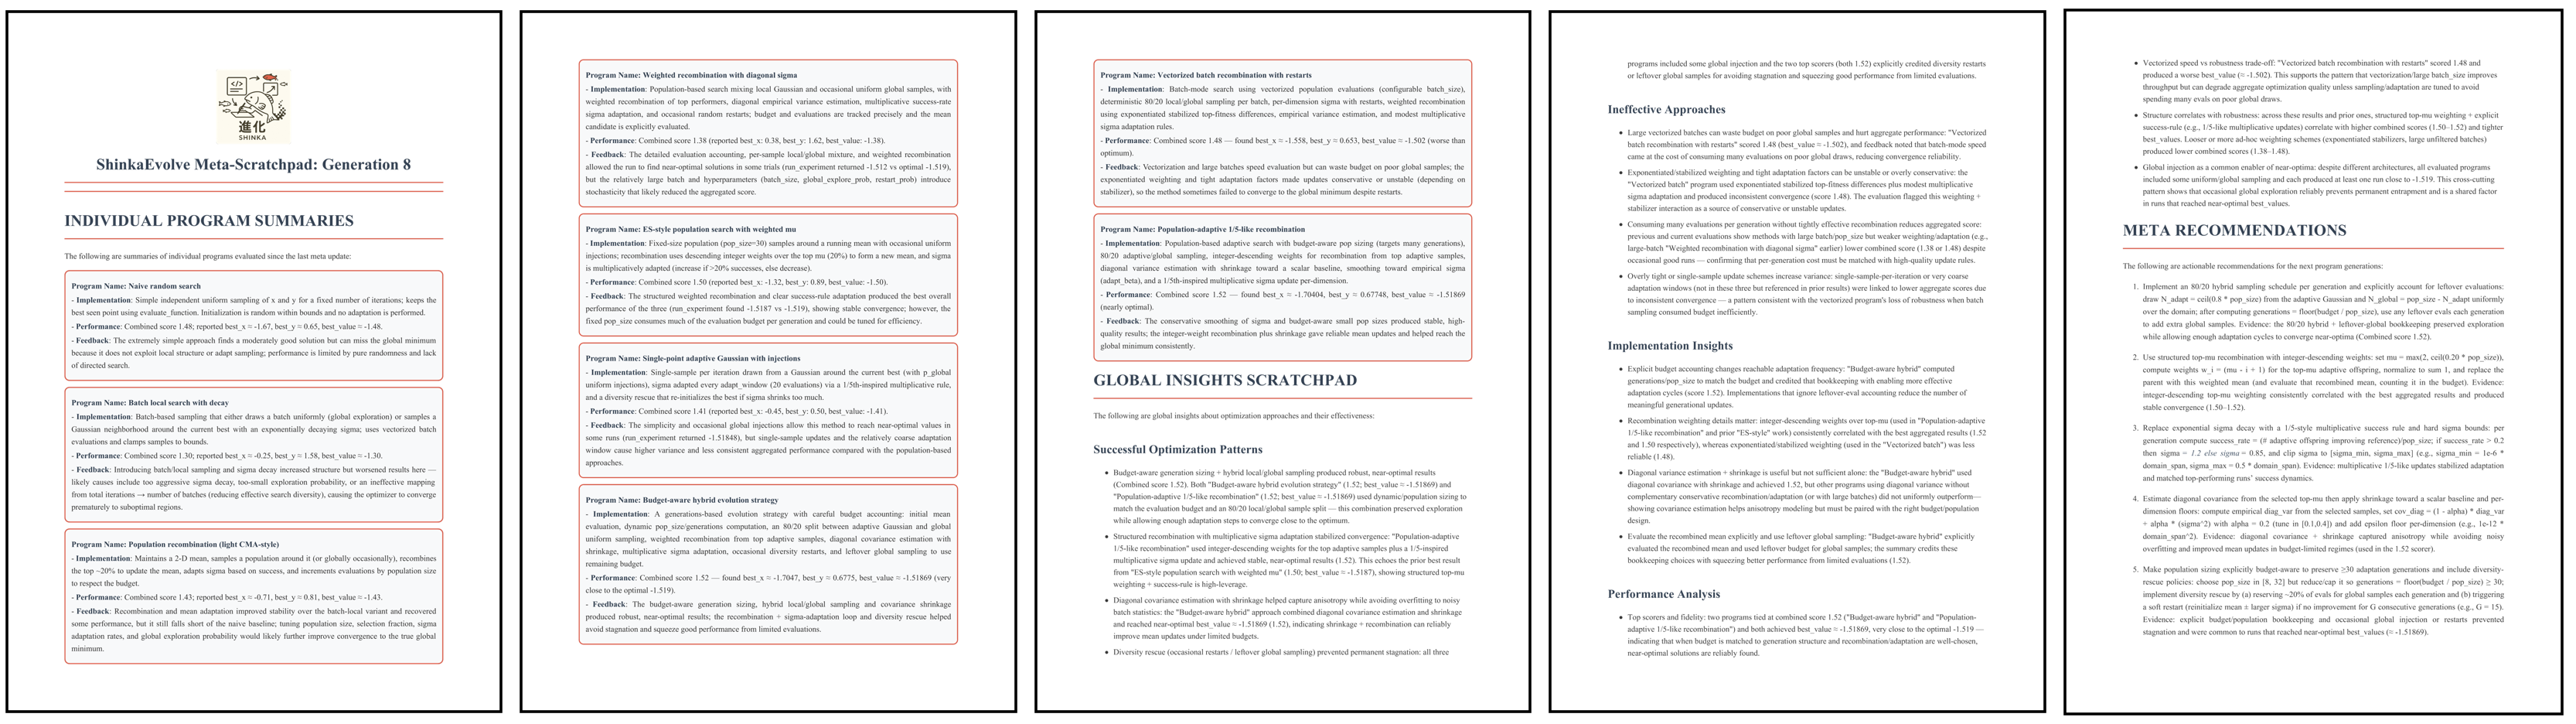
\includegraphics[width=0.9\textwidth]{figures/f2_c_scratchpad.png}
    \caption{\textbf{A \ouralgo Meta-Scratchpad.} It consists of individual program summaries, global insights, and implementation recommendations, which are appended to the mutation prompt.}
    \label{fig:meta_scratchpad}
\end{figure}